%%%% Paramétrage du TD %%%%
\def\xxactivite{Révisions \ifprof -- Corrigé \else \fi} % \normalsize \vspace{-.4cm}
\def\xxauteur{\textsl{Xavier Pessoles}}


\def\xxnumchapitre{Chapitre 1 \vspace{.2cm}}
\def\xxchapitre{\hspace{.12cm} Correction des systèmes}


\def\xxcompetences{%
\vspace{-.3cm}
\textsl{%
\textbf{Savoirs et compétences :}\\
%\vspace{-.4cm}
%\begin{itemize}[label=\ding{112},font=\color{ocre}] 
%%\item \textit{Res1.C4 : } Correction
% \item \textit{Res1.C4.SF1 : } Proposer la démarche de réglage d’un correcteur proportionnel
%%proportionnel intégral 
%%et à avance de phase
%\item \textit{Con.C2 : } 	Correction d’un système asservi	
%\item \textit{Con.C2.SF1 : } Choisir un type de correcteur adapté
%\end{itemize}
}}

\def\xxauteur{\textsl{Xavier Pessoles}}

\def\xxtitreexo{TD -- Révisions de cinématique \ifnormal $\star$ \else \fi \iftdifficile $\star\star\star$ \else \fi }
\def\xxsourceexo{}%\hspace{.2cm} \footnotesize{Concours CCP -- PSI 2018}}

\def\xxfigures{
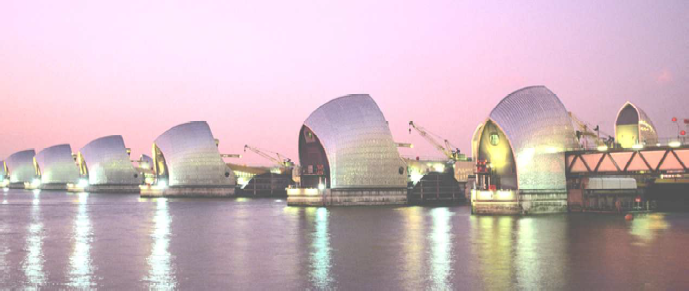
\includegraphics[width=.6\linewidth]{fig1}
}%figues de la page de garde

\def\xxpied{%
Révision cinématique -- Modélisation cinématique\\
\xxactivite%
}

\iflivret
\pagestyle{empty}


%%%%%%%% PAGE DE GARDE COURS
\ifcours
% ==== BANDEAU DES TITRES ==== 
\begin{tikzpicture}[remember picture,overlay]
\node at (current page.north west)
{\begin{tikzpicture}[remember picture,overlay]
\node[anchor=north west,inner sep=0pt] at (0,0) {\includegraphics[width=\paperwidth]{\thechapterimage}};
\draw[anchor=west] (-2cm,-8cm) node [line width=2pt,rounded corners=15pt,draw=ocre,fill=white,fill opacity=0.6,inner sep=40pt]{\strut\makebox[22cm]{}};
\draw[anchor=west] (1cm,-8cm) node {\huge\sffamily\bfseries\color{black} %
\begin{minipage}{1cm}
\rotatebox{90}{\LARGE\sffamily\textsc{\color{ocre}\textbf{\xxnumpartie}}}
\end{minipage} \hfill
\begin{minipage}[c]{14cm}
\begin{titrepartie}
\begin{flushright}
\renewcommand{\baselinestretch}{1.1} 
\Large\sffamily\textsc{\textbf{\xxpartie}}
\renewcommand{\baselinestretch}{1} 
\end{flushright}
\end{titrepartie}
\end{minipage} \hfill
\begin{minipage}[c]{3.5cm}
{\large\sffamily\textsc{\textbf{\color{ocre} \discipline}}}
\end{minipage} 
 };
\end{tikzpicture}};
\end{tikzpicture}
% ==== FIN BANDEAU DES TITRES ==== 


% ==== ONGLET 
\begin{tikzpicture}[overlay]
\node[shape=rectangle, 
      rounded corners = .25 cm,
	  draw= ocre,
	  line width=2pt, 
	  fill = ocre!10,
	  minimum width  = 2.5cm,
	  minimum height = 3cm,] at (18.3cm,0) {};
\node at (17.7cm,0) {\rotatebox{90}{\textbf{\Large\color{ocre}{\classe}}}};
%{};
\end{tikzpicture}
% ==== FIN ONGLET 


\vspace{3.5cm}

\begin{tikzpicture}[remember picture,overlay]
\draw[anchor=west] (-2cm,-6cm) node {\huge\sffamily\bfseries\color{black} %
\begin{minipage}{2cm}
\begin{center}
\LARGE\sffamily\textsc{\color{ocre}\textbf{\xxactivite}}
\end{center}
\end{minipage} \hfill
\begin{minipage}[c]{15cm}
\begin{titrechapitre}
\renewcommand{\baselinestretch}{1.1} 
\Large\sffamily\textsc{\textbf{\xxnumchapitre}}

\Large\sffamily\textsc{\textbf{\xxchapitre}}
\vspace{.5cm}

\renewcommand{\baselinestretch}{1} 
\normalsize\normalfont
\xxcompetences
\end{titrechapitre}
\end{minipage}  };
\end{tikzpicture}
\vfill

\begin{flushright}
\begin{minipage}[c]{.3\linewidth}
\begin{center}
\xxfigures
\end{center}
\end{minipage}\hfill
\begin{minipage}[c]{.6\linewidth}
\startcontents
%\printcontents{}{1}{}
\printcontents{}{1}{}
\end{minipage}
\end{flushright}

\begin{tikzpicture}[remember picture,overlay]
\draw[anchor=west] (4.5cm,-.7cm) node {
\begin{minipage}[c]{.2\linewidth}
\begin{flushright}

\includegraphics[width=2cm]{logoCC}
\end{flushright}
\end{minipage}
\begin{minipage}[c]{.2\linewidth}
\textsl{\xxauteur} \\
\textsl{\classe}
\end{minipage}
 };
\end{tikzpicture}

\newpage
\pagestyle{fancy}

%\newpage
%\pagestyle{fancy}

\else
\fi
%% FIN PAGE DE GARDE DES COURS

%%%%%%%% PAGE DE GARDE TD
\iftd
%\begin{tikzpicture}[remember picture,overlay]
%\node at (current page.north west)
%{\begin{tikzpicture}[remember picture,overlay]
%\draw[anchor=west] (-2cm,-3.25cm) node [line width=2pt,rounded corners=15pt,draw=ocre,fill=white,fill opacity=0.6,inner sep=40pt]{\strut\makebox[22cm]{}};
%\draw[anchor=west] (1cm,-3.25cm) node {\huge\sffamily\bfseries\color{black} %
%\begin{minipage}{1cm}
%\rotatebox{90}{\LARGE\sffamily\textsc{\color{ocre}\textbf{\xxnumpartie}}}
%\end{minipage} \hfill
%\begin{minipage}[c]{13.5cm}
%\begin{titrepartie}
%\begin{flushright}
%\renewcommand{\baselinestretch}{1.1} 
%\Large\sffamily\textsc{\textbf{\xxpartie}}
%\renewcommand{\baselinestretch}{1} 
%\end{flushright}
%\end{titrepartie}
%\end{minipage} \hfill
%\begin{minipage}[c]{3.5cm}
%{\large\sffamily\textsc{\textbf{\color{ocre} \discipline}}}
%\end{minipage} 
% };
%\end{tikzpicture}};
%\end{tikzpicture}

%%%%%%%%%% PAGE DE GARDE TD %%%%%%%%%%%%%%%
%\begin{tikzpicture}[overlay]
%\node[shape=rectangle, 
%      rounded corners = .25 cm,
%	  draw= ocre,
%	  line width=2pt, 
%	  fill = ocre!10,
%	  minimum width  = 2.5cm,
%	  minimum height = 2.5cm,] at (18.5cm,0) {};
%\node at (17.7cm,0) {\rotatebox{90}{\textbf{\Large\color{ocre}{\classe}}}};
%%{};
%\end{tikzpicture}

% PARTIE ET CHAPITRE
%\begin{tikzpicture}[remember picture,overlay]
%\draw[anchor=west] (-1cm,-2.1cm) node {\large\sffamily\bfseries\color{black} %
%\begin{minipage}[c]{15cm}
%\begin{flushleft}
%\xxnumchapitre \\
%\xxchapitre
%\end{flushleft}
%\end{minipage}  };
%\end{tikzpicture}

% BANDEAU EXO
\iflivret % SI LIVRET
\begin{tikzpicture}[remember picture,overlay]
\draw[anchor=west] (-2cm,-3.3cm) node {\huge\sffamily\bfseries\color{black} %
\begin{minipage}{5cm}
\begin{center}
\LARGE\sffamily\color{ocre}\textbf{\textsc{\xxactivite}}

\begin{center}
\xxfigures
\end{center}

\end{center}
\end{minipage} \hfill
\begin{minipage}[c]{12cm}
\begin{titrechapitre}
\renewcommand{\baselinestretch}{1.1} 
\large\sffamily\textbf{\textsc{\xxtitreexo}}

\small\sffamily{\textbf{\textit{\color{black!70}\xxsourceexo}}}
\vspace{.5cm}

\renewcommand{\baselinestretch}{1} 
\normalsize\normalfont
\xxcompetences
\end{titrechapitre}
\end{minipage}};
\end{tikzpicture}
\else % ELSE NOT LIVRET
\begin{tikzpicture}[remember picture,overlay]
\draw[anchor=west] (-2cm,-4.5cm) node {\huge\sffamily\bfseries\color{black} %
\begin{minipage}{5cm}
\begin{center}
\LARGE\sffamily\color{ocre}\textbf{\textsc{\xxactivite}}

\begin{center}
\xxfigures
\end{center}

\end{center}
\end{minipage} \hfill
\begin{minipage}[c]{12cm}
\begin{titrechapitre}
\renewcommand{\baselinestretch}{1.1} 
\large\sffamily\textbf{\textsc{\xxtitreexo}}

\small\sffamily{\textbf{\textit{\color{black!70}\xxsourceexo}}}
\vspace{.5cm}

\renewcommand{\baselinestretch}{1} 
\normalsize\normalfont
\xxcompetences
\end{titrechapitre}
\end{minipage}};
\end{tikzpicture}

\fi

\else   % FIN IF TD
\fi


%%%%%%%% PAGE DE GARDE FICHE
\iffiche
\begin{tikzpicture}[remember picture,overlay]
\node at (current page.north west)
{\begin{tikzpicture}[remember picture,overlay]
\draw[anchor=west] (-2cm,-2.25cm) node [line width=2pt,rounded corners=15pt,draw=ocre,fill=white,fill opacity=0.6,inner sep=40pt]{\strut\makebox[22cm]{}};
\draw[anchor=west] (1cm,-2.25cm) node {\huge\sffamily\bfseries\color{black} %
\begin{minipage}{1cm}
\rotatebox{90}{\LARGE\sffamily\textsc{\color{ocre}\textbf{\xxnumpartie}}}
\end{minipage} \hfill
\begin{minipage}[c]{14cm}
\begin{titrepartie}
\begin{flushright}
\renewcommand{\baselinestretch}{1.1} 
\large\sffamily\textsc{\textbf{\xxpartie} \\} 

\vspace{.2cm}

\normalsize\sffamily\textsc{\textbf{\xxnumchapitre -- \xxchapitre}}
\renewcommand{\baselinestretch}{1} 
\end{flushright}
\end{titrepartie}
\end{minipage} \hfill
\begin{minipage}[c]{3.5cm}
{\large\sffamily\textsc{\textbf{\color{ocre} \discipline}}}
\end{minipage} 
 };
\end{tikzpicture}};
\end{tikzpicture}

\iflivret
\begin{tikzpicture}[overlay]
\node[shape=rectangle, 
      rounded corners = .25 cm,
	  draw= ocre,
	  line width=2pt, 
	  fill = ocre!10,
	  minimum width  = 2.5cm,
	  minimum height = 2.5cm,] at (18.5cm,.5cm) {};
\node at (17.9cm,.5cm) {\rotatebox{90}{\textsf{\textbf{\large\color{ocre}{\classe}}}}};
%{};
\end{tikzpicture}
\else
\begin{tikzpicture}[overlay]
\node[shape=rectangle, 
      rounded corners = .25 cm,
	  draw= ocre,
	  line width=2pt, 
	  fill = ocre!10,
	  minimum width  = 2.5cm,
%	  minimum height = 2.5cm,] at (18.5cm,1.1cm) {};
	  minimum height = 2.5cm,] at (18.6cm,0.5cm) {};
\node at (18cm,0.5cm) {\rotatebox{90}{\textsf{\textbf{\large\color{ocre}{\classe}}}}};
%{};
\end{tikzpicture}

\fi

\else
\fi



\else
\pagestyle{empty}


%%%%%%%% PAGE DE GARDE COURS
\ifcours
% ==== BANDEAU DES TITRES ==== 
\begin{tikzpicture}[remember picture,overlay]
\node at (current page.north west)
{\begin{tikzpicture}[remember picture,overlay]
\node[anchor=north west,inner sep=0pt] at (0,0) {\includegraphics[width=\paperwidth]{\thechapterimage}};
\draw[anchor=west] (-2cm,-8cm) node [line width=2pt,rounded corners=15pt,draw=ocre,fill=white,fill opacity=0.6,inner sep=40pt]{\strut\makebox[22cm]{}};
\draw[anchor=west] (1cm,-8cm) node {\huge\sffamily\bfseries\color{black} %
\begin{minipage}{1cm}
\rotatebox{90}{\LARGE\sffamily\textsc{\color{ocre}\textbf{\xxnumpartie}}}
\end{minipage} \hfill
\begin{minipage}[c]{14cm}
\begin{titrepartie}
\begin{flushright}
\renewcommand{\baselinestretch}{1.1} 
\Large\sffamily\textsc{\textbf{\xxpartie}}
\renewcommand{\baselinestretch}{1} 
\end{flushright}
\end{titrepartie}
\end{minipage} \hfill
\begin{minipage}[c]{3.5cm}
{\large\sffamily\textsc{\textbf{\color{ocre} \discipline}}}
\end{minipage} 
 };
\end{tikzpicture}};
\end{tikzpicture}
% ==== FIN BANDEAU DES TITRES ==== 


% ==== ONGLET 
\begin{tikzpicture}[overlay]
\node[shape=rectangle, 
      rounded corners = .25 cm,
	  draw= ocre,
	  line width=2pt, 
	  fill = ocre!10,
	  minimum width  = 2.5cm,
	  minimum height = 3cm,] at (18.3cm,0) {};
\node at (17.7cm,0) {\rotatebox{90}{\textbf{\Large\color{ocre}{\classe}}}};
%{};
\end{tikzpicture}
% ==== FIN ONGLET 


\vspace{3.5cm}

\begin{tikzpicture}[remember picture,overlay]
\draw[anchor=west] (-2cm,-6cm) node {\huge\sffamily\bfseries\color{black} %
\begin{minipage}{2cm}
\begin{center}
\LARGE\sffamily\textsc{\color{ocre}\textbf{\xxactivite}}
\end{center}
\end{minipage} \hfill
\begin{minipage}[c]{15cm}
\begin{titrechapitre}
\renewcommand{\baselinestretch}{1.1} 
\Large\sffamily\textsc{\textbf{\xxnumchapitre}}

\Large\sffamily\textsc{\textbf{\xxchapitre}}
\vspace{.5cm}

\renewcommand{\baselinestretch}{1} 
\normalsize\normalfont
\xxcompetences
\end{titrechapitre}
\end{minipage}  };
\end{tikzpicture}
\vfill

\begin{flushright}
\begin{minipage}[c]{.3\linewidth}
\begin{center}
\xxfigures
\end{center}
\end{minipage}\hfill
\begin{minipage}[c]{.6\linewidth}
\startcontents
%\printcontents{}{1}{}
\printcontents{}{1}{}
\end{minipage}
\end{flushright}

\begin{tikzpicture}[remember picture,overlay]
\draw[anchor=west] (4.5cm,-.7cm) node {
\begin{minipage}[c]{.2\linewidth}
\begin{flushright}

\includegraphics[width=2cm]{logoCC}
\end{flushright}
\end{minipage}
\begin{minipage}[c]{.2\linewidth}
\textsl{\xxauteur} \\
\textsl{\classe}
\end{minipage}
 };
\end{tikzpicture}

\newpage
\pagestyle{fancy}

%\newpage
%\pagestyle{fancy}

\else
\fi
%% FIN PAGE DE GARDE DES COURS

%%%%%%%% PAGE DE GARDE TD
\iftd
%\begin{tikzpicture}[remember picture,overlay]
%\node at (current page.north west)
%{\begin{tikzpicture}[remember picture,overlay]
%\draw[anchor=west] (-2cm,-3.25cm) node [line width=2pt,rounded corners=15pt,draw=ocre,fill=white,fill opacity=0.6,inner sep=40pt]{\strut\makebox[22cm]{}};
%\draw[anchor=west] (1cm,-3.25cm) node {\huge\sffamily\bfseries\color{black} %
%\begin{minipage}{1cm}
%\rotatebox{90}{\LARGE\sffamily\textsc{\color{ocre}\textbf{\xxnumpartie}}}
%\end{minipage} \hfill
%\begin{minipage}[c]{13.5cm}
%\begin{titrepartie}
%\begin{flushright}
%\renewcommand{\baselinestretch}{1.1} 
%\Large\sffamily\textsc{\textbf{\xxpartie}}
%\renewcommand{\baselinestretch}{1} 
%\end{flushright}
%\end{titrepartie}
%\end{minipage} \hfill
%\begin{minipage}[c]{3.5cm}
%{\large\sffamily\textsc{\textbf{\color{ocre} \discipline}}}
%\end{minipage} 
% };
%\end{tikzpicture}};
%\end{tikzpicture}

%%%%%%%%%% PAGE DE GARDE TD %%%%%%%%%%%%%%%
%\begin{tikzpicture}[overlay]
%\node[shape=rectangle, 
%      rounded corners = .25 cm,
%	  draw= ocre,
%	  line width=2pt, 
%	  fill = ocre!10,
%	  minimum width  = 2.5cm,
%	  minimum height = 2.5cm,] at (18.5cm,0) {};
%\node at (17.7cm,0) {\rotatebox{90}{\textbf{\Large\color{ocre}{\classe}}}};
%%{};
%\end{tikzpicture}

% PARTIE ET CHAPITRE
%\begin{tikzpicture}[remember picture,overlay]
%\draw[anchor=west] (-1cm,-2.1cm) node {\large\sffamily\bfseries\color{black} %
%\begin{minipage}[c]{15cm}
%\begin{flushleft}
%\xxnumchapitre \\
%\xxchapitre
%\end{flushleft}
%\end{minipage}  };
%\end{tikzpicture}

% BANDEAU EXO
\iflivret % SI LIVRET
\begin{tikzpicture}[remember picture,overlay]
\draw[anchor=west] (-2cm,-3.3cm) node {\huge\sffamily\bfseries\color{black} %
\begin{minipage}{5cm}
\begin{center}
\LARGE\sffamily\color{ocre}\textbf{\textsc{\xxactivite}}

\begin{center}
\xxfigures
\end{center}

\end{center}
\end{minipage} \hfill
\begin{minipage}[c]{12cm}
\begin{titrechapitre}
\renewcommand{\baselinestretch}{1.1} 
\large\sffamily\textbf{\textsc{\xxtitreexo}}

\small\sffamily{\textbf{\textit{\color{black!70}\xxsourceexo}}}
\vspace{.5cm}

\renewcommand{\baselinestretch}{1} 
\normalsize\normalfont
\xxcompetences
\end{titrechapitre}
\end{minipage}};
\end{tikzpicture}
\else % ELSE NOT LIVRET
\begin{tikzpicture}[remember picture,overlay]
\draw[anchor=west] (-2cm,-4.5cm) node {\huge\sffamily\bfseries\color{black} %
\begin{minipage}{5cm}
\begin{center}
\LARGE\sffamily\color{ocre}\textbf{\textsc{\xxactivite}}

\begin{center}
\xxfigures
\end{center}

\end{center}
\end{minipage} \hfill
\begin{minipage}[c]{12cm}
\begin{titrechapitre}
\renewcommand{\baselinestretch}{1.1} 
\large\sffamily\textbf{\textsc{\xxtitreexo}}

\small\sffamily{\textbf{\textit{\color{black!70}\xxsourceexo}}}
\vspace{.5cm}

\renewcommand{\baselinestretch}{1} 
\normalsize\normalfont
\xxcompetences
\end{titrechapitre}
\end{minipage}};
\end{tikzpicture}

\fi

\else   % FIN IF TD
\fi


%%%%%%%% PAGE DE GARDE FICHE
\iffiche
\begin{tikzpicture}[remember picture,overlay]
\node at (current page.north west)
{\begin{tikzpicture}[remember picture,overlay]
\draw[anchor=west] (-2cm,-2.25cm) node [line width=2pt,rounded corners=15pt,draw=ocre,fill=white,fill opacity=0.6,inner sep=40pt]{\strut\makebox[22cm]{}};
\draw[anchor=west] (1cm,-2.25cm) node {\huge\sffamily\bfseries\color{black} %
\begin{minipage}{1cm}
\rotatebox{90}{\LARGE\sffamily\textsc{\color{ocre}\textbf{\xxnumpartie}}}
\end{minipage} \hfill
\begin{minipage}[c]{14cm}
\begin{titrepartie}
\begin{flushright}
\renewcommand{\baselinestretch}{1.1} 
\large\sffamily\textsc{\textbf{\xxpartie} \\} 

\vspace{.2cm}

\normalsize\sffamily\textsc{\textbf{\xxnumchapitre -- \xxchapitre}}
\renewcommand{\baselinestretch}{1} 
\end{flushright}
\end{titrepartie}
\end{minipage} \hfill
\begin{minipage}[c]{3.5cm}
{\large\sffamily\textsc{\textbf{\color{ocre} \discipline}}}
\end{minipage} 
 };
\end{tikzpicture}};
\end{tikzpicture}

\iflivret
\begin{tikzpicture}[overlay]
\node[shape=rectangle, 
      rounded corners = .25 cm,
	  draw= ocre,
	  line width=2pt, 
	  fill = ocre!10,
	  minimum width  = 2.5cm,
	  minimum height = 2.5cm,] at (18.5cm,.5cm) {};
\node at (17.9cm,.5cm) {\rotatebox{90}{\textsf{\textbf{\large\color{ocre}{\classe}}}}};
%{};
\end{tikzpicture}
\else
\begin{tikzpicture}[overlay]
\node[shape=rectangle, 
      rounded corners = .25 cm,
	  draw= ocre,
	  line width=2pt, 
	  fill = ocre!10,
	  minimum width  = 2.5cm,
%	  minimum height = 2.5cm,] at (18.5cm,1.1cm) {};
	  minimum height = 2.5cm,] at (18.6cm,0.5cm) {};
\node at (18cm,0.5cm) {\rotatebox{90}{\textsf{\textbf{\large\color{ocre}{\classe}}}}};
%{};
\end{tikzpicture}

\fi

\else
\fi



\fi
\setlength{\columnseprule}{.1pt}

\pagestyle{fancy}
\thispagestyle{plain}

\vspace{5cm}

\def\columnseprulecolor{\color{ocre}}
\setlength{\columnseprule}{0.4pt} 

\setcounter{exo}{0}

\ifprof
%\begin{multicols}{2}
\else
\begin{multicols}{2}
\fi
%%%%%%%%%%%%%%%%%%%%%%%%%%%%%%%%%%%%%%%%%%%%%%%%%%




\section*{Pales d'hélicoptères}
\subsection*{Mise en situation}
%\vspace{.5cm}
\ifprof
\else
%\begin{minipage}[c]{.6\linewidth}
%\begin{center}
%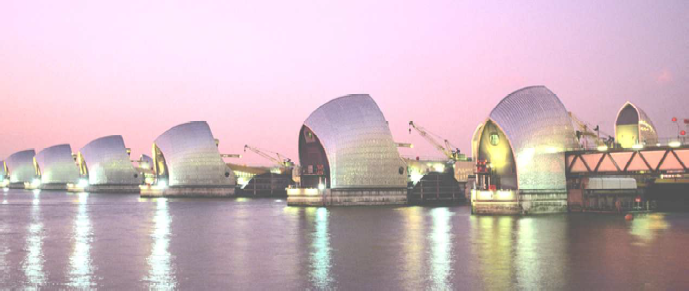
\includegraphics[width=.7\linewidth]{fig1}
%\end{center}
L'hélicoptère est un giravion dont la sustentation est assurée par un rotor primaire équipé de pales. Un rotor secondaire (ou rotor de queue, lui aussi équipé de pales) permet à l'hélicoptère de ne pas tourner sur lui même. Ces rotors sont entraînés par une ou deux turbines suivant les hélicoptères, par l'intermédiaire d'une boîte de vitesse. 

En vol, les rotors tournent à une vitesse de rotation fixe. La modification de l'inclinaison des pales permet à elle seule une accélération, un décélération, un changement d'altitude ou de direction de l'hélicoptère.

%\end{minipage} \hfill
%\begin{minipage}[c]{.35\linewidth}

%\end{minipage}

\begin{center}
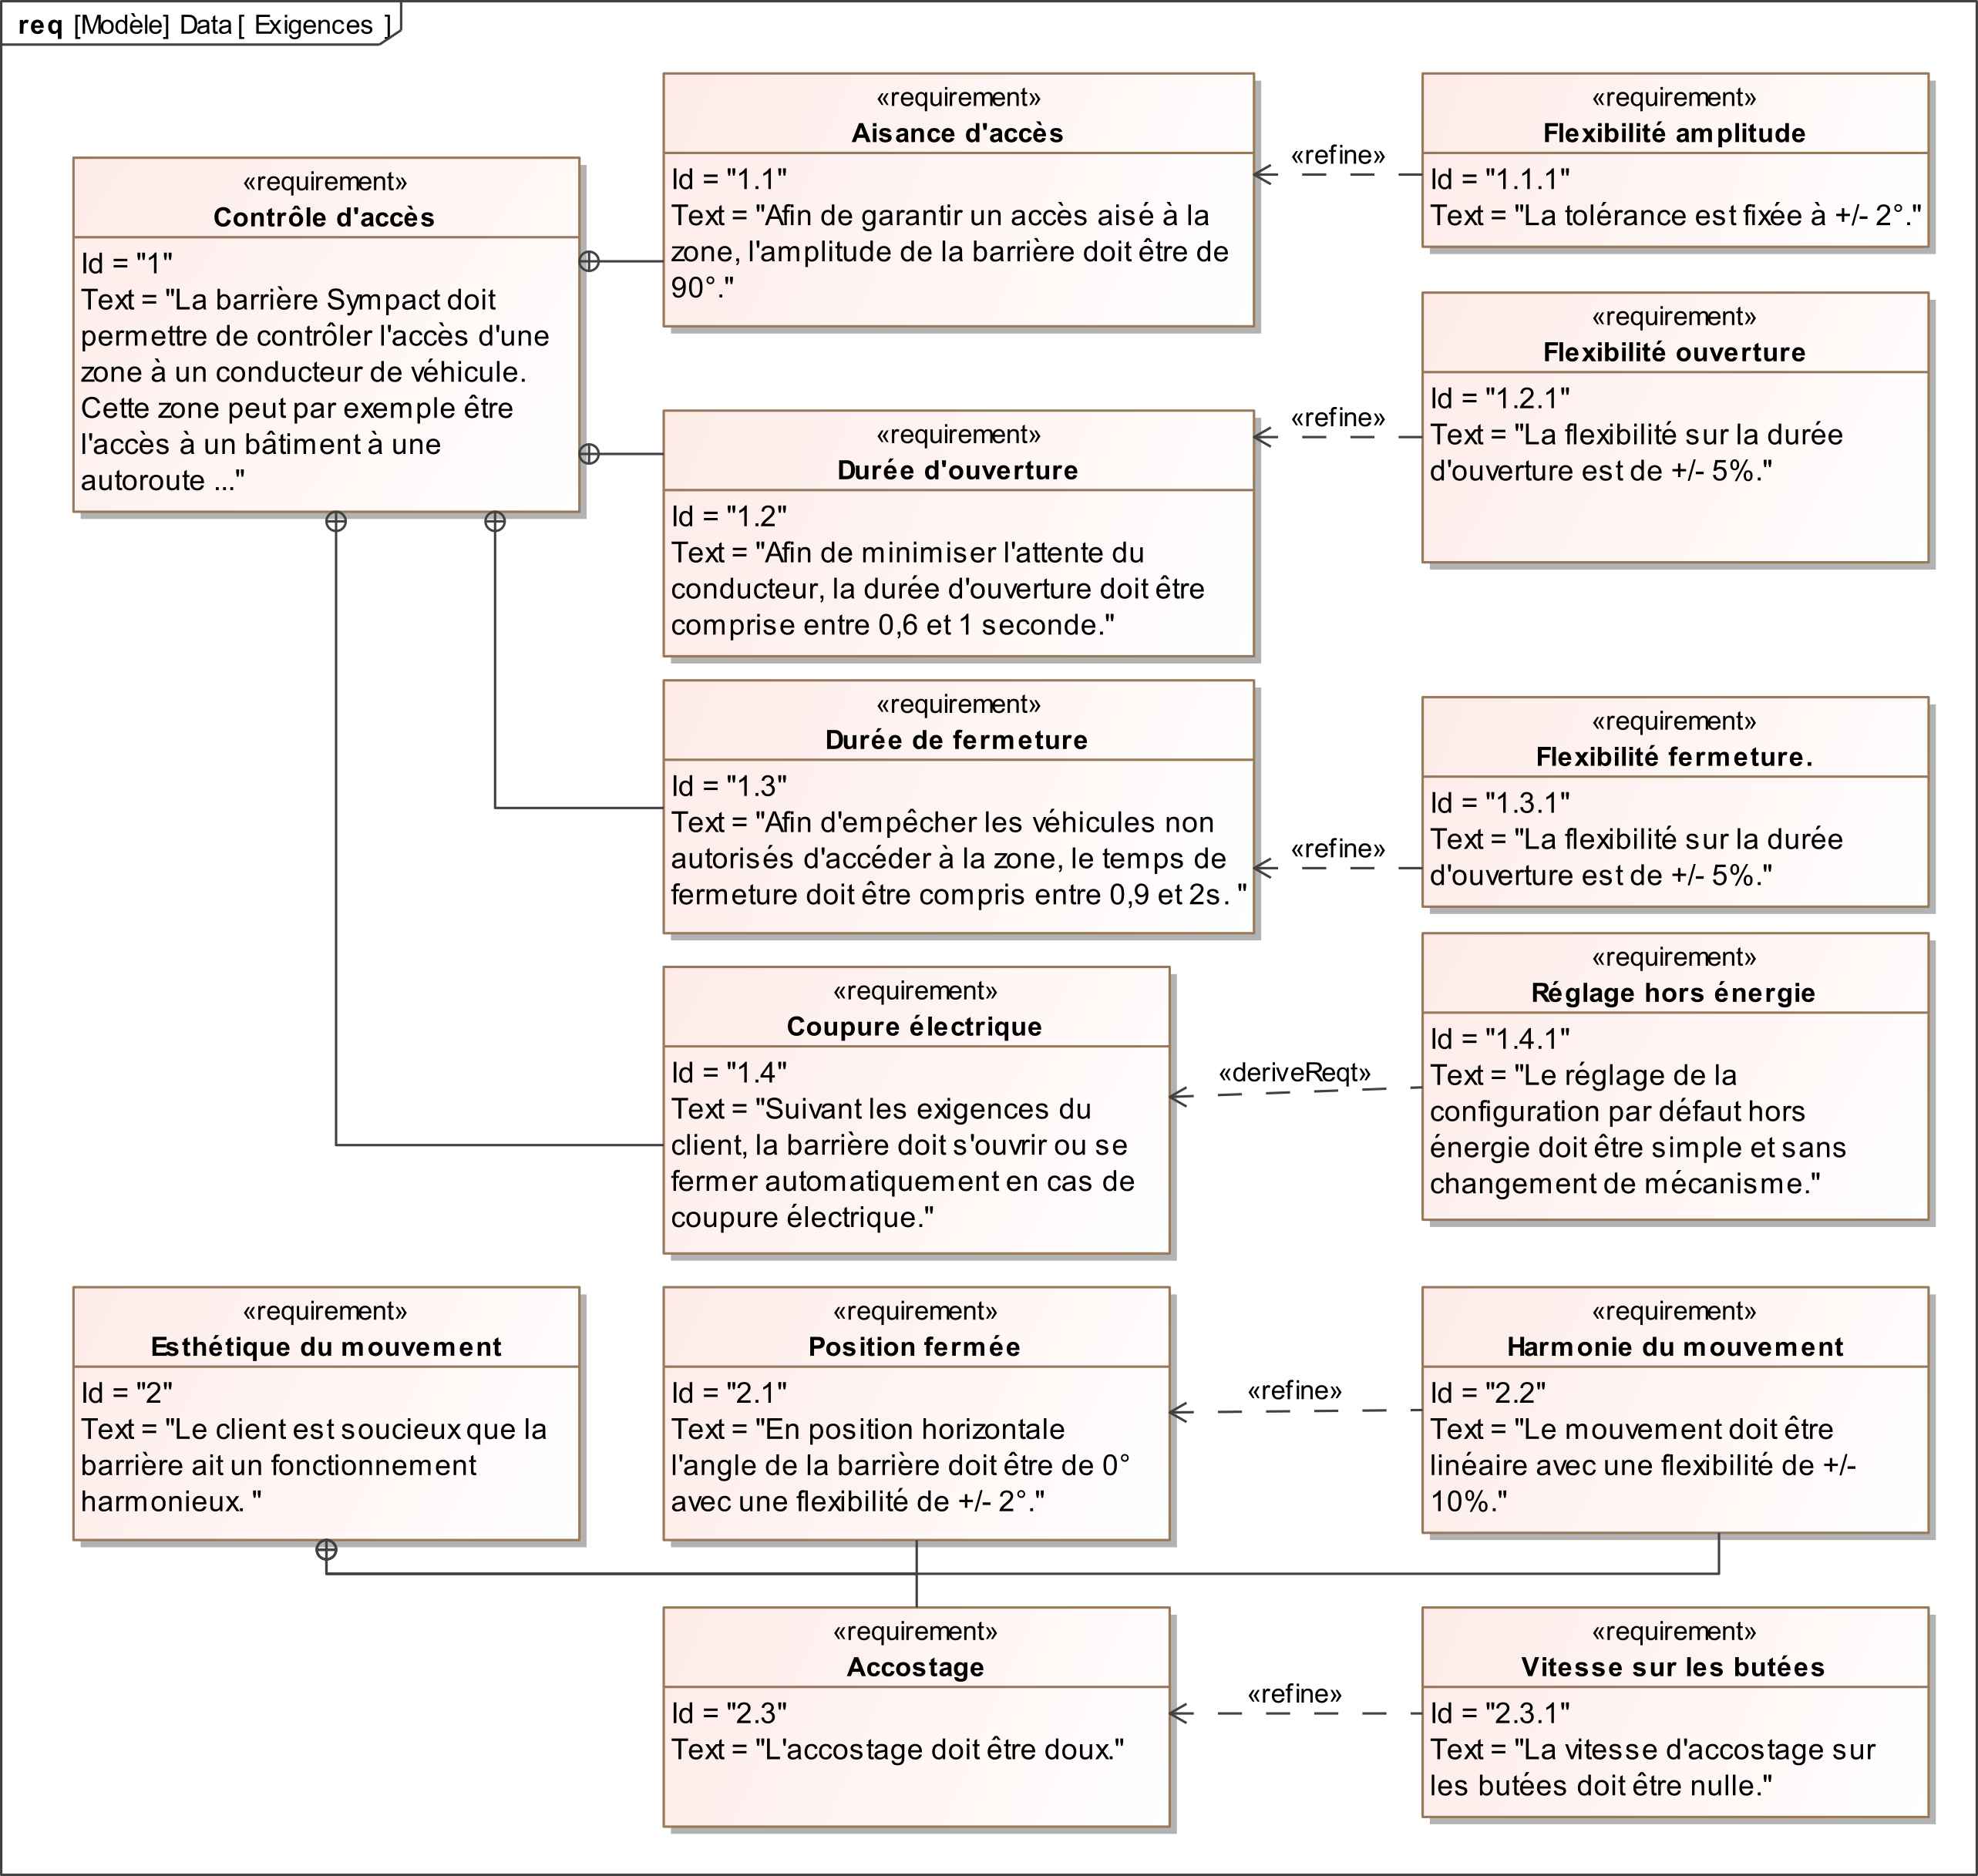
\includegraphics[width=\linewidth]{SysML/Exigences}
\end{center}
%}
\fi
\subsection*{Cinématique analytique}
\ifprof
\else
\begin{center}
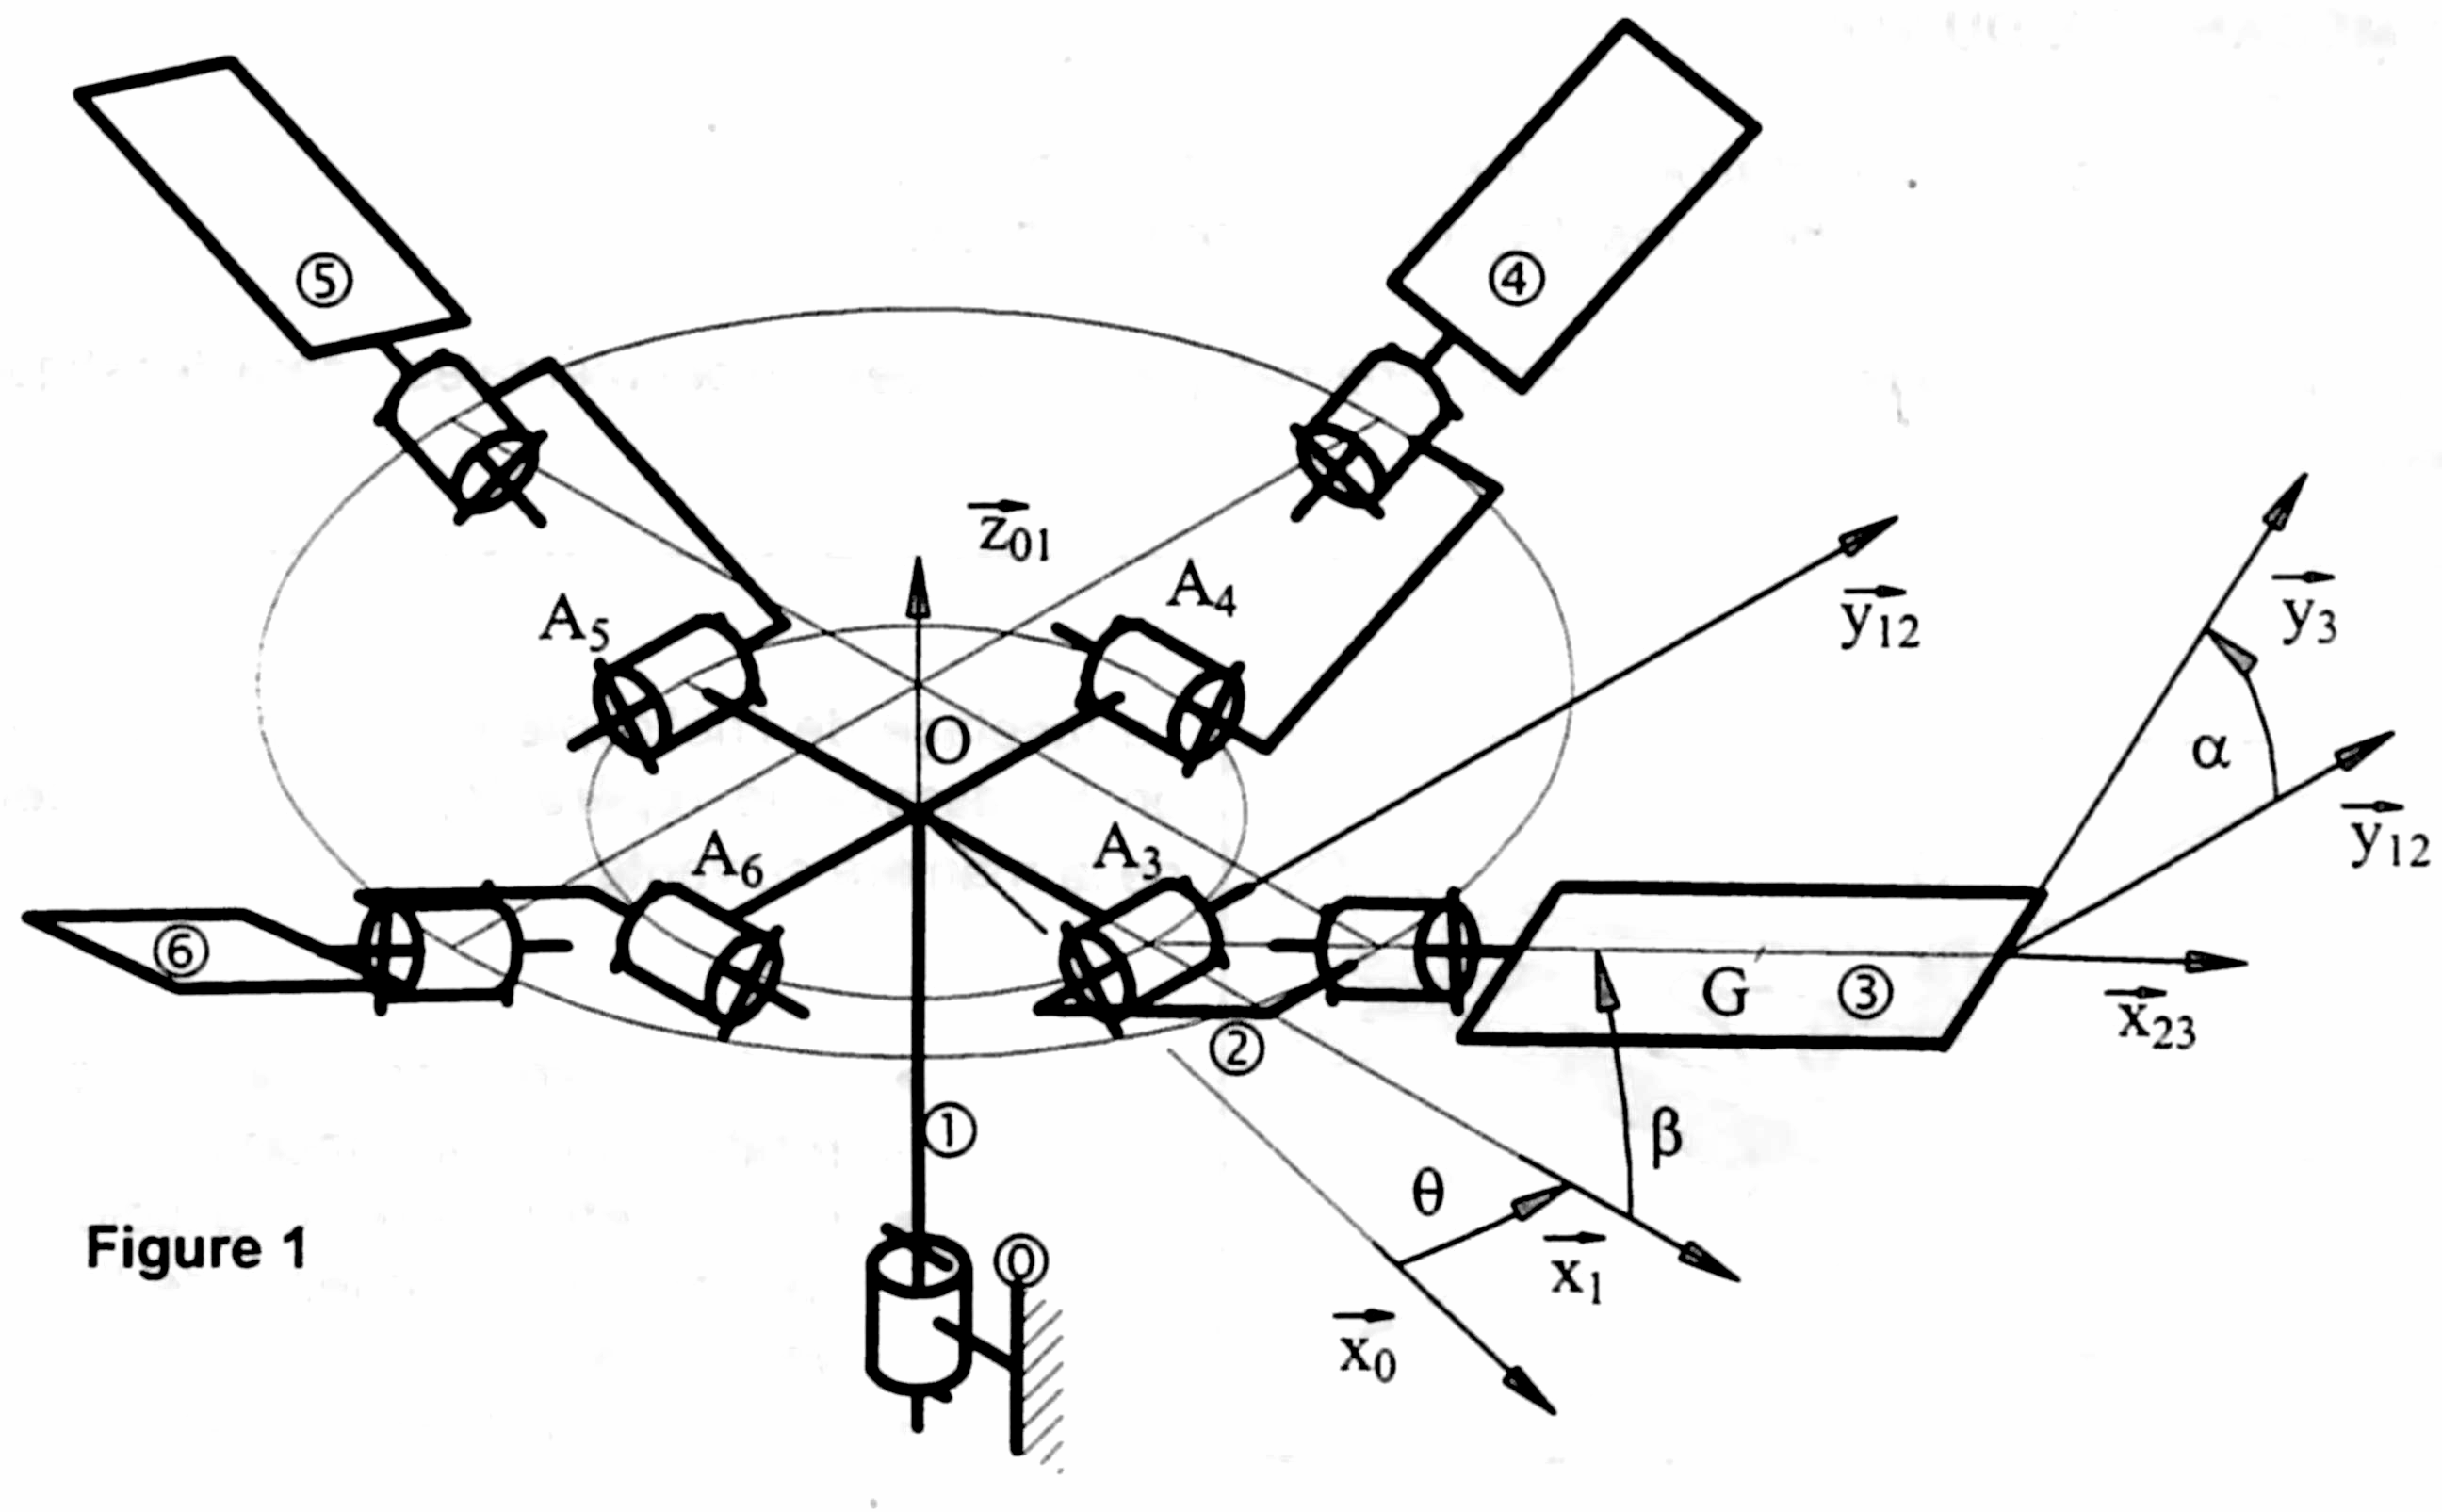
\includegraphics[width=.8\linewidth]{fig2}
\end{center}

Le fuselage de l'hélicoptère est repéré par $S_0$ et on lui associe le repère $\mathcal{R}_0(O,\vect{x_0},\vect{y_0},\vect{z_{01}})$ défini de la
manière suivante :
\begin{itemize}
\item $(O,\vect{z_{01}})$ correspond à l'axe de rotation du rotor principal;
\item $(O, \vect{x_0} )$ définit l'axe longitudinal de l'appareil et est orienté de l'arrière vers l'avant;
\item $(O, \vect{y_0} )$ définit l'axe transversal.
\end{itemize}

Ce rotor est constitué de :
\begin{itemize}
\item un moyeu central $S_1$ associé au repère $\mathcal{R}_1(O,\vect{x_1},\vect{y_{12}},\vect{z_{01}})$ qui est entraîné par la boîte de vitesse (non
représentée ici);
\item quatre pales $S_3$, $S_4$, $S_5$ et $S_6$. On associe le repère $\mathcal{R}_3(A_3,\vect{x_{23}},\vect{y_3},\vect{z_3} )$ à la pale $S_3$;
\item quatre pieds de pales identiques reliant les pales au moyeu. On associe le repère
$\mathcal{R}_2(A3,\vect{x_{23}},\vect{y_{12}},\vect{z_2} )$ au pied de pale $S_2$.
\end{itemize}

NB : Si les repères $\mathcal{R}_i$ et $\mathcal{R}_j$ ont un vecteur de base commun (par exemple $\vect{x_i}= \vect{x_j}$ ), celui-ci est noté $\vect{x_{ij}}$.


Le mouvement de $S_1/S_0$ est une rotation d'axe $(O,\vect{z_{01}})$. On pose $\theta$ l’angle de rotation du rotor : $\theta = (\vect{x_0},\vect{x_1})$ .

Le mouvement de $S_2/S_1$ est une rotation d'axe $(A_3,\vect{y_{12}})$ . On pose $\beta$ l’angle de battement : $\beta = (\vect{x_1},\vect{x_{23}})$.

Le mouvement de $S_3/S_2$ est une rotation d'axe $(A_3,\vect{x_{23}})$. On pose $\alpha$ l’angle de pas : $\alpha = (\vect{y_{12}},\vect{y_3})$.

On pose $\vect{OA_3} = r\cdot \vect{x_1}$ et $\vect{A_3G}=a\cdot \vect{x_{23}}$ où $G$ est le centre de gravité de la pale 3 ($r$ et $a$ constants). On suppose que tous les solides sont indéformables.


\begin{center}
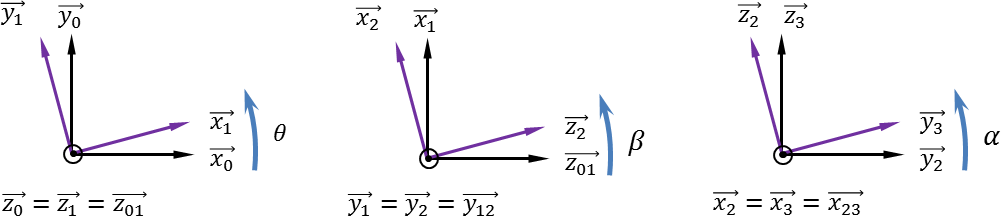
\includegraphics[width=.9\linewidth]{cor1}
\end{center}

\fi
%\subparagraph{}
%\textit{Réaliser 3 figures planes illustrant les 3 paramètres d'orientation $\theta$, $\beta$ et $\alpha$ , puis en déduire le vecteur rotation traduisant chaque figure.}
%\ifprof
%\begin{corrige}
%\begin{center}
%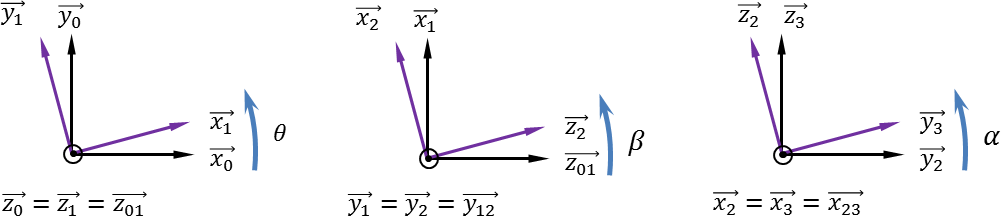
\includegraphics[width=.9\linewidth]{cor1}
%\end{center}
%\end{corrige}\else \fi

\subparagraph{}
%\textit{Déterminer le torseur $\torseurcin{V}{S_3}{S_2}$ au point $G$.}
\textit{Déterminer le vecteur $\vectv{G}{S_3}{S_2}$.}
\ifprof
\begin{corrige}
On a: 
$$
\torseurcin{V}{S_3}{S_2} = \torseurl{\vecto{S_3}{S_2}=\dot{\alpha}\vect{x_{23}}}{\vectv{A_3}{S_3}{S_2}=\vect{0}}{A_3}
$$

Par ailleurs, $
\vectv{G}{S_3}{S_2}=\underbrace{\vectv{A_3}{S_3}{S_2}}_{\vect{0}}+\vect{GA_3}\wedge\vecto{S_3}{S_2}$
$=
-a\vect{x_{23}}\wedge \dot{\alpha}\vect{x_{23}}=\vect{0}
$.

Au final, 
$$
\torseurcin{V}{S_3}{S_2} = \torseurl{\vecto{S_3}{S_2}=\dot{\alpha}\vect{x_{23}}}{\vectv{G}{S_3}{S_2}=\vect{0}}{G}
$$

\end{corrige}
\else \fi

\subparagraph{}
%\textit{Déterminer le torseur $\torseurcin{V}{S_2}{S_1}$ au point $G$.}
\textit{Déterminer le vecteur $\vectv{G}{S_2}{S_1}$.}
\ifprof
\begin{corrige}
On a: 
$$
\torseurcin{V}{S_2}{S_1} = \torseurl{\vecto{S_2}{S_1}=\dot{\beta}\vect{y_{12}}}{\vectv{A_3}{S_2}{S_1}=\vect{0}}{A_3}
$$

Par ailleurs, 
$
\vectv{G}{S_2}{S_1}=\underbrace{\vectv{A_3}{S_2}{S_1}}_{\vect{0}}+\vect{GA_3}\wedge\vecto{S_2}{S_1}$
$=
-a\vect{x_{23}}\wedge \dot{\beta}\vect{y_{12}}=-a\dot{\beta}\vect{z_{2}}
$

Au final, 
$$
\torseurcin{V}{S_2}{S_1} = \torseurl{\vecto{S_2}{S_1}=\dot{\beta}\vect{y_{12}}}{\vectv{G}{S_2}{S_1}=-a\dot{\beta}\vect{z_{2}}}{G}
$$\end{corrige}\else \fi

\subparagraph{}
%\textit{Déterminer le torseur $\torseurcin{V}{S_1}{S_0}$ au point $G$.}
\textit{Déterminer le vecteur $\vectv{G}{S_1}{S_0}$.}
\ifprof
\begin{corrige}
On a: 
$$
\torseurcin{V}{S_1}{S_0} = \torseurl{\vecto{S_1}{S_0}=\dot{\theta}\vect{z_{01}}}{\vectv{O}{S_1}{S_0}=\vect{0}}{O}
$$

Par ailleurs, 
$
\vectv{G}{S_1}{S_0}=\underbrace{\vectv{O}{S_1}{S_0}}_{\vect{0}}+\vect{GO}\wedge\vecto{S_1}{S_0}$
$=
\left(-a\vect{x_{23}}-r\vect{x_1}\right)\wedge \dot{\theta}\vect{z_{01}}=
a\dot{\theta}\cos\beta\vect{y_{12}}+r\dot{\theta}\vect{y_{12}}
$

Au final, 
$$
\torseurcin{V}{S_1}{S_0} = 
\torseurl{
\vecto{S_1}{S_0}=\dot{\theta}\vect{z_{01}}
}{%
\vectv{G}{S_1}{S_0}
=\dot{\theta}\left(a\cos\beta+r\right)\vect{y_{12}}}{G}
$$

\end{corrige}\else \fi

\subparagraph{}
%\textit{En déduire $\torseurcin{V}{S_3}{S_0}$ au point $G$.}
\textit{Déduire des questions précédentes le torseur $\torseurcin{V}{S_3}{S_0}$ au point $G$.}

\ifprof
\begin{corrige}
Par composition du torseur cinématique on a :
$$
\torseurcin{V}{S_3}{S_0} = 
\torseurcin{V}{S_3}{S_2} + \torseurcin{V}{S_2}{S_1} + \torseurcin{V}{S_1}{S_0}
$$

Tous les torseurs ayant déjà été exprimés au même point, on a :
$$
\torseurcin{V}{S_3}{S_0} = 
\torseurl{
\vecto{S_3}{S_0}=\dot{\theta}\vect{z_{01}}+\dot{\alpha}\vect{x_{23}}
+\dot{\beta}\vect{y_{12}}
}{%
\vectv{G}{S_3}{S_0}
=\dot{\theta}\left(a\cos\beta+r\right)\vect{y_{12}}-a\dot{\beta}\vect{z_{2}}}{G}
$$

On pose maintenant $\vectv{G}{S_3}{S_0}=(a \cdot \cos \beta + r) \cdot \dot{\theta} \cdot \vect{y_{12}}-a\dot{\beta}\vect{z_2}$.
\end{corrige}\else \fi


On pose maintenant $\vectv{G}{S_3}{S_0}=(a \cdot \cos \beta + r) \cdot \dot{\theta} \cdot \vect{y_{12}}-a\dot{\beta}\vect{z_2}$.

\subparagraph{}
\textit{Exprimer l'accélération $\vectg{G}{S_3}{S_0}$.}
\ifprof
\begin{corrige}
Par définition, 
$$
\vectg{G}{S_3}{S_0} = 
\left[
\dfrac{\vectv{G}{S_3}{S_0}}{dt}
\right]_{\mathcal{R}_0}
$$

Il est donc nécessaire de dériver $\vect{y_{12}}$ et $\vect{z_{2}}$ :
$$
\left[
\dfrac{d\vect{y_{12}}}{dt}
\right]_{\mathcal{R}_0}
=
\left[
\dfrac{d\vect{y_{12}}}{dt}
\right]_{\mathcal{R}_1}+\vecto{S_1}{S_0} \wedge \vect{y_{12}}
=\dot{\theta}\vect{z_{01}} \wedge \vect{y_{12}}
=-\dot{\theta}\vect{x_{1}}
$$

$$
\left[
\dfrac{d\vect{z_{2}}}{dt}
\right]_{\mathcal{R}_0}
=
\left[
\dfrac{d\vect{z_{2}}}{dt}
\right]_{\mathcal{R}_2}+\vecto{S_2}{S_0} \wedge \vect{z_{2}}
=\left(
\dot{\theta}\vect{z_{01}}+\dot{\beta}\vect{y_{12}}
\right) \wedge \vect{z_{2}}
=
\dot{\theta}\sin\beta\vect{y_1}
+\dot{\beta}\vect{x_{2}}
$$

Au final :
$$
\vectg{G}{S_3}{S_0} = 
-a \dot{\beta} \sin \beta \dot{\theta} \vect{y_{12}}
+(a \cos \beta + r) \ddot{\theta} \vect{y_{12}}
-(a \cos \beta + r) \dot{\theta}^2 \vect{x_{1}}
-a\ddot{\beta}\vect{z_2}
-a\dot{\beta}\left( \dot{\theta}\sin\beta\vect{y_1}
+\dot{\beta}\vect{x_{2}}\right)
$$
\end{corrige}\else \fi

\subparagraph{}
\textit{La longueur des pales est, entre autre, limitée par la vitesse du son en bout de pale (Exigence 1.1.1.1.1). Pour $\beta=0$, calculer la longueur maximale de la pale pour ne pas dépasser la vitesse du son. La vitesse du rotor est de $\SI{250}{tr.min^{-1}}$.}
\ifprof
\begin{corrige}
Lorsque $\beta=0$ la vitesse en bout de pale est donnée par $L\dot{\theta}$.
$\dot{\theta}=250 \; tr/min = \dfrac{250 \cdot 2 \pi}{60}\;rad/s = 26,18\;rad/s$
On a donc :
$$
L = \dfrac{295,1}{26,18} =\SI{11,2}{m}
$$
\end{corrige}\else \fi

\section*{Système de coffre motorisé}
\setcounter{subparagraph}{0}
\begin{flushleft}
\textit{D'après le concours Centrale -- Supélec 2007.}
\end{flushleft}
\ifprof
\else

\begin{center}
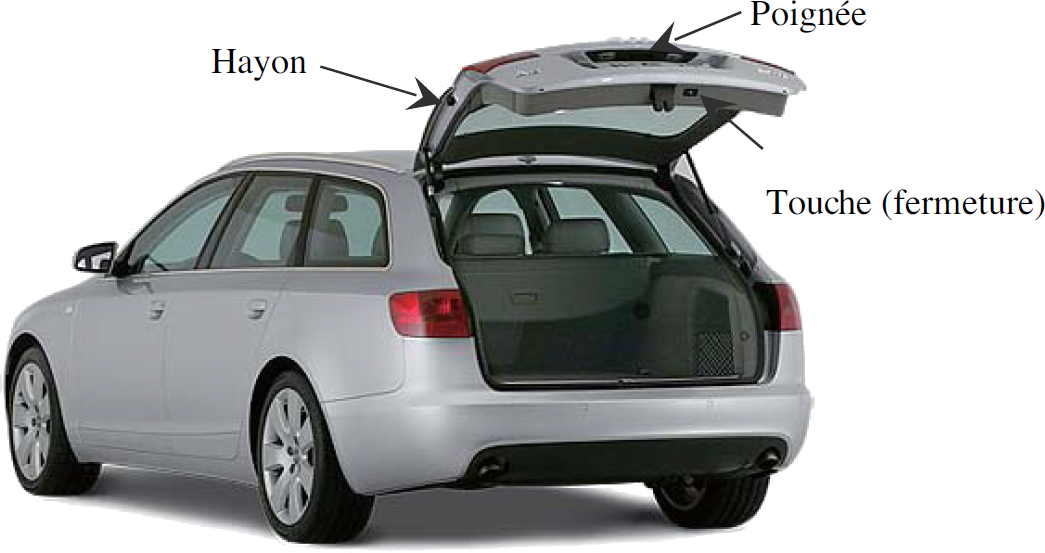
\includegraphics[width=.7\linewidth]{A6_coffre}
\end{center}

%\ifprof
%\noindent\begin{minipage}[c]{.55\linewidth}
Depuis 2005, un coffre motorisé est proposé en option sur l’Audi A6. La motorisation du hayon permet l’ouverture ou la fermeture automatique du coffre. L’ouverture s’effectue soit à l’aide de la télécommande, soit par action sur une touche située à proximité du conducteur, soit par action sur une touche située sur la poignée du hayon. La fermeture s’effectue par action sur une touche située sur la face interne du hayon.

%\end{minipage} \hfill
%\begin{minipage}[c]{.43\linewidth}

%\end{minipage}}

\begin{obj}
\begin{itemize}
\item Vérifier le rapport de réduction du train épicycloïdal.
\item Déterminer la loi Entrée -- Sortie du système 4 barres.
\end{itemize}
\end{obj}

%\begin{minipage}[c]{.4\linewidth}
L’utilisateur a la possibilité de programmer l’angle d’ouverture du hayon pour
éviter par exemple qu’il ne heurte le plafond du garage. L’utilisateur conserve
naturellement la possibilité de man\oe{}uvrer manuellement le hayon. Ce système
dispose également de détecteurs d’obstacles.
En position fermée, le système doit assurer le blocage du hayon avec la caisse
du véhicule.
%\end{minipage}\hfill
%\begin{minipage}[c]{.59\linewidth}
\begin{center}
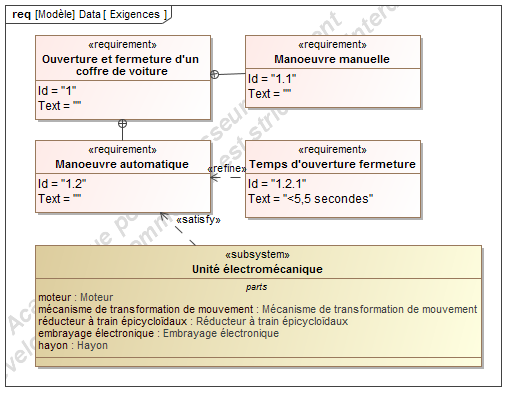
\includegraphics[width=.95\linewidth]{SysML/Req}
\end{center}

%\end{minipage}


La chaîne d'énergie du système est constituée :
\begin{itemize}
\item d'un moteur à courant continu;
\item d'un embrayage électromagnétique;
\item d'un double train épicycloïdal
\item d'un mécanisme de transformation de mouvement de type 4 barres;
\item de l'effecteur à savoir le hayon \textbf{45} du coffre.
\end{itemize}

\begin{center}
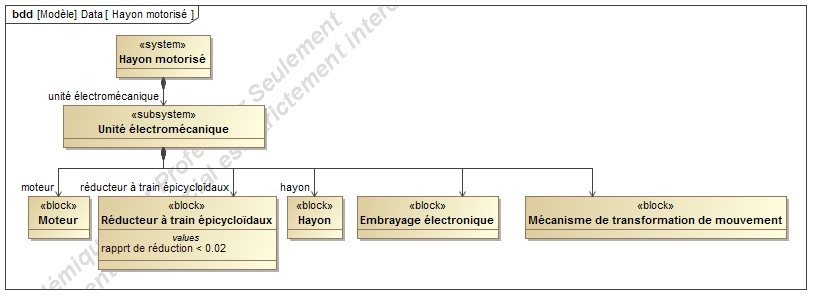
\includegraphics[width=.95\linewidth]{SysML/BDD}
\end{center}


\begin{center}
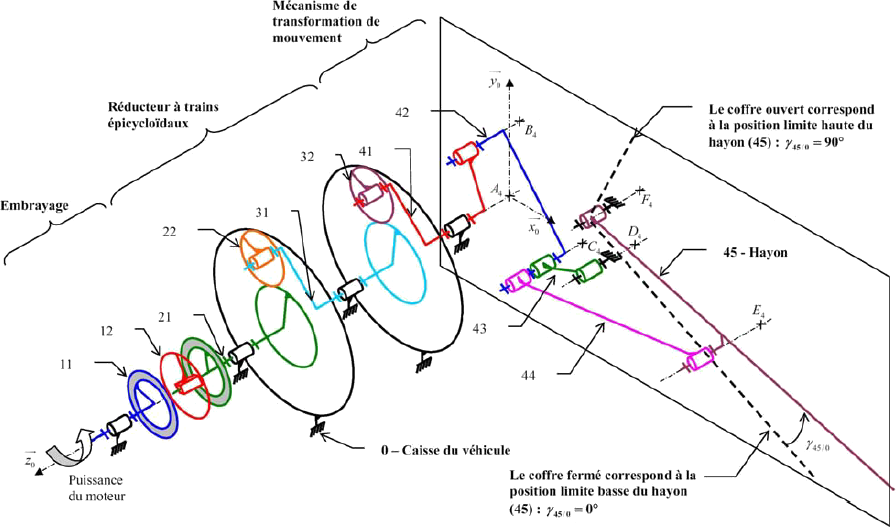
\includegraphics[width=.95\linewidth]{A6_schema}
\end{center}

\fi

\subsection*{Étude du train épicycloïdal}
\ifprof
\else

On donne le schéma cinématique du double train épicycloïdal. 

%\vspace{.25cm}

%\begin{minipage}[c]{.6\linewidth}
Le premier train est constitué :
\begin{itemize}
\item du planétaire \textbf{21}. On note $\vecto{21}{0}=\omega(21/0)\vect{z_0}$ et $||\vect{IA}|| =R_{21} $;
\item du satellite \textbf{22}. On note $\vecto{22}{31}=\omega(22/31)\vect{z_0}$ et $||\vect{IB}|| =R_{22}$;
\item du porte-satellite \textbf{31}. On note $\vecto{31}{0}=\omega(31/0)\vect{z_0}$;
\item de la couronne \textbf{0}. On note  $||\vect{AJ}|| =R_{0}$;.
\end{itemize}
%\end{minipage}\hfill
%\begin{minipage}[c]{.37\linewidth}
Le second train est constitué :
\begin{itemize}
\item du planétaire \textbf{21};
\item du satellite \textbf{32};
\item du porte-satellite \textbf{41};
\item de la couronne \textbf{0}.
\end{itemize}
%\end{minipage}


\fi


\begin{center}
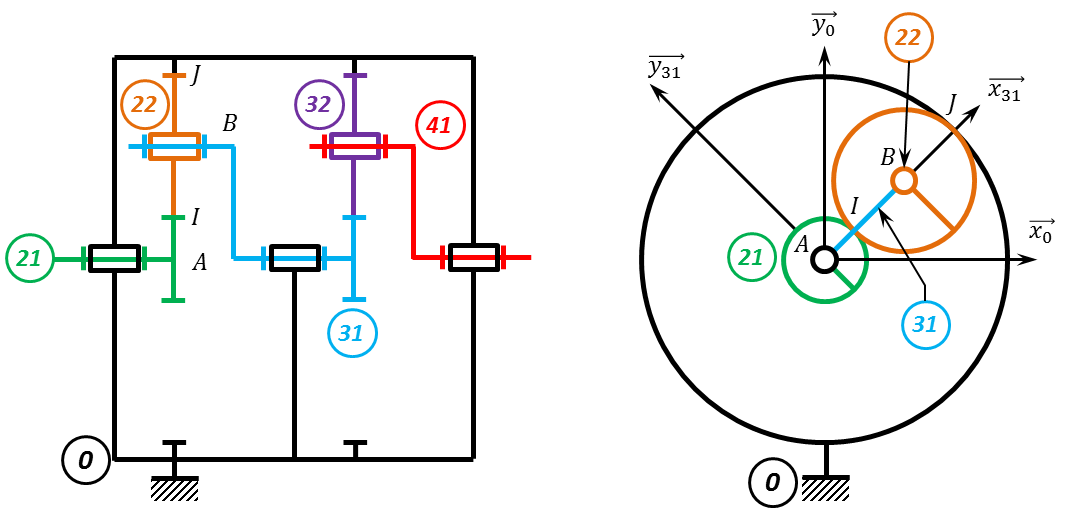
\includegraphics[width=\linewidth]{A6_train}
\end{center}

\subparagraph{}
\textit{Déterminer le rapport de réduction $\dfrac{\omega(31/0)}{\omega(21/0)}$.}
\ifprof
\begin{corrige}
On bloque le porte-satellite 31 et on libère le bâti. On a $\dfrac{\omega(0/31)}{\omega(21/31)}=-\dfrac{Z_{21}}{Z_0}$.

On cherche 
$\dfrac{\omega(31/0)}{\omega(21/0)}$; donc $\dfrac{\omega(31/0)}{\omega(21/31)}=\dfrac{\omega(31/0)}{\omega(21/0)+\omega(0/31)}=\dfrac{Z_{21}}{Z_0}$
$\Leftrightarrow \omega(31/0)=\dfrac{Z_{21}}{Z_0}\omega(21/0)-\dfrac{Z_{21}}{Z_0}\omega(31/0)$
$\Leftrightarrow \omega(31/0)\left(1+\dfrac{Z_{21}}{Z_0}\right)=\dfrac{Z_{21}}{Z_0}\omega(21/0)$
$\Leftrightarrow \dfrac{\omega(31/0)}{\omega(21/0)}=\dfrac{\dfrac{Z_{21}}{Z_0}}{1+\dfrac{Z_{21}}{Z_0}}=\dfrac{Z_{21}}{Z_{0}+Z_{21}}$
\end{corrige}
\else
\fi

\subparagraph{}
\textit{Déterminer le rapport de réduction $\dfrac{\omega(41/0)}{\omega(31/0)}$.}
\ifprof
\begin{corrige}
Par analogie, 
$\dfrac{\omega(41/0)}{\omega(31/0)}=\dfrac{Z_{31}}{Z_{0}+Z_{31}}$
\end{corrige}
\else
\fi


%\subparagraph{}
%\textit{Après avoir exprimé la relation de roulement sans glissement au point $I$, montrer que $R_{22} \omega(22/31) = R_{21} \left( \omega(31/0) - \omega(21/0)\right)$. }
%\ifprof
%\begin{corrige}
%En faisant l'hypothèse que \textbf{22} roule sans glisser sur \textbf{21}, on a : 
%$$ 
%\vectv{I}{22}{21} = \vect{0}
%$$
%On a alors : 
%$$
%\vectv{I}{22}{31} + \vectv{I}{31}{0}+\vectv{I}{0}{21} = \vect{0}
%\Longleftrightarrow
%\vectv{I}{22}{31} + \vectv{I}{31}{0}-\vectv{I}{21}{0} = \vect{0}$$
%
%\footnotesize
%\noindent\begin{minipage}[c]{.3\linewidth}
%\begin{eqnarray*}
%&&\vectv{I}{22}{31} \\
%&=& \vectv{B}{22}{31} + \vect{IB} \wedge \vecto{22}{31}\\
%&=& R_{22}\vect{x_{31}} \wedge \omega(22/31)\vect{z_0} \\
%&=& - R_{22} \omega(22/31)\vect{y_{31}}
%\end{eqnarray*}
%\end{minipage} \hfill
%\begin{minipage}[c]{.3\linewidth}
%\begin{eqnarray*}
%&&\vectv{I}{31}{0} \\
%&=& \vectv{A}{31}{0} + \vect{IA} \wedge \vecto{31}{0}\\
%&=&  -R_{21}\vect{x_{31}} \wedge \omega(31/0)\vect{z_0} \\
%&=& R_{21} \omega(31/0)\vect{y_{31}}
%\end{eqnarray*}
%\end{minipage} \hfill
%\begin{minipage}[c]{.3\linewidth}
%\begin{eqnarray*}
%&&\vectv{I}{21}{0}\\
%&=& \vectv{A}{31}{0} + \vect{IA} \wedge \vecto{31}{0}\\
%&=& -R_{21}\vect{x_{31}} \wedge \omega(21/0)\vect{z_0} \\
%&=&  R_{21} \omega(21/0)\vect{y_{31}}
%\end{eqnarray*}
%\end{minipage}
%
%\normalsize
%
%\vspace{.25cm}
%On a donc :
%
%$$- R_{22} \omega(22/31)\vect{y_{31}} + R_{21} \omega(31/0)\vect{y_{31}}
%-  R_{21} \omega(21/0)\vect{y_{31}}= \vect{0}
%$$
%
%$$
%\Longrightarrow
%- R_{22} \omega(22/31) + R_{21} \omega(31/0) -  R_{21} \omega(21/0)= 0
%\Longleftrightarrow
%R_{22} \omega(22/31) = R_{21} \left( \omega(31/0) - \omega(21/0)\right)
%$$
%
%\end{corrige}
%\else \fi
%
%\subparagraph{}
%\textit{Après avoir exprimé la relation de roulement sans glissement au point $J$, déterminer une relation entre $R_{22}$, $\omega(22/31)$, $R_{0}$ et $\omega(31/0)$.}
%\ifprof
%\begin{corrige}
%En faisant l'hypothèse que \textbf{22} roule sans glisser sur \textbf{0}, on a : 
%$$ 
%\vectv{J}{22}{0} = \vect{0}
%\Longleftrightarrow \vectv{J}{22}{31} + \vectv{J}{31}{0} = \vect{0}
%$$
%
%\noindent\begin{minipage}[c]{.45\linewidth}
%\begin{eqnarray*}
%&&\vectv{J}{22}{31} \\
%&=& \vectv{B}{22}{31} + \vect{JB} \wedge \vecto{22}{31}\\
%&=& - R_{22}\vect{x_{31}} \wedge \omega(22/31)\vect{z_0} \\
%&=&  R_{22} \omega(22/31)\vect{y_{31}}
%\end{eqnarray*}
%\end{minipage} \hfill
%\begin{minipage}[c]{.45\linewidth}
%\begin{eqnarray*}
%&&\vectv{J}{31}{0} \\
%&=& \vectv{A}{31}{0} + \vect{JA} \wedge \vecto{31}{0}\\
%&=&  -R_{0}\vect{x_{31}} \wedge \omega(31/0)\vect{z_0} \\
%&=& R_{0} \omega(31/0)\vect{y_{31}}
%\end{eqnarray*}
%\end{minipage} 
%
%\vspace{.25cm}
%
%On a donc :
%
%$$R_{22} \omega(22/31)\vect{y_{31}} +R_{0} \omega(31/0)\vect{y_{31}}= \vect{0}
%\Longrightarrow
%R_{22} \omega(22/31) +R_{0} \omega(31/0)= 0
%$$
%
%\end{corrige}
%\else \fi
%
%
%\subparagraph{}
%\textit{Déterminer alors le rapport de réduction $\dfrac{\omega(31/0)}{\omega(21/0)}$.}
%
%\ifprof
%\begin{corrige}
%On a : 
%$$
%R_{22} \omega(22/31) = R_{21} \left( \omega(31/0) - \omega(21/0)\right) 
%\quad \text{et} \quad
%R_{22} \omega(22/31) +R_{0} \omega(31/0)= 0
%$$
%
%Au final :
%$$
% R_{21} \omega(21/0)= R_{21} \omega(31/0) + R_{0} \omega(31/0)
%\Longleftrightarrow
%\dfrac{\omega(31/0)}{\omega(21/0)} = \dfrac{R_{21}}{R_{21}+R_{0}}
%= \dfrac{Z_{21}}{Z_{21}+Z_{0}}
%$$
%
%Par ailleurs, la condition d'entraxe dans un train épicycoïdal se formule ainsi : 
%$AJ = AI+IJ \Longleftrightarrow R_0 = R_{21} + 2 R_{22}$. On a alors : 
%$$
%\dfrac{\omega(31/0)}{\omega(21/0)} 
%= \dfrac{Z_{21}}{2 Z_{21}+Z_{22}}
%$$
%
%\end{corrige}
%\else \fi


\subparagraph{}
\textit{En déduire le rapport de réduction du double train épicycloïdal. Puis faire l'application numérique. On donne $Z_{21}=13$ et $Z_{22}=81$. Le rapport de réduction est-il compatible avec celui du diagramme de blocs ?}

\ifprof
\begin{corrige}

Le rapport de réduction du réducteur s'exprime par : 
$\dfrac{Z_{21}}{Z_{0}+Z_{21}}\dfrac{Z_{31}}{Z_{0}+Z_{31}}$. Si les deux trains ont les mêmes caractéristiques, on a $\left(\dfrac{Z_{21}}{Z_{0}+Z_{21}}\right)^2$. 
En exprimant les conditions de fonctionnement, on a : 
$R_{21}+2R_{22}=R_0\Leftrightarrow Z_{21}+2Z_{22}=Z_0$. %et $R_{31}+2R_{32}=R_0$. En conséquences, 
%$R_{21}+2R_{22}=R_{31}+2R_{32}$ $\Longleftrightarrow Z_{21}+2Z_{22}=Z_{31}+2Z_{32}$. 

On a : alors 
$$
\left(\dfrac{Z_{21}}{2 Z_{21}+2Z_{22}}\right)^2=0,0047%0,0147
$$
\end{corrige}
\else \fi

\subsection*{Étude du mécanisme de transformation de mouvement}

\ifprof
\else

\begin{center}
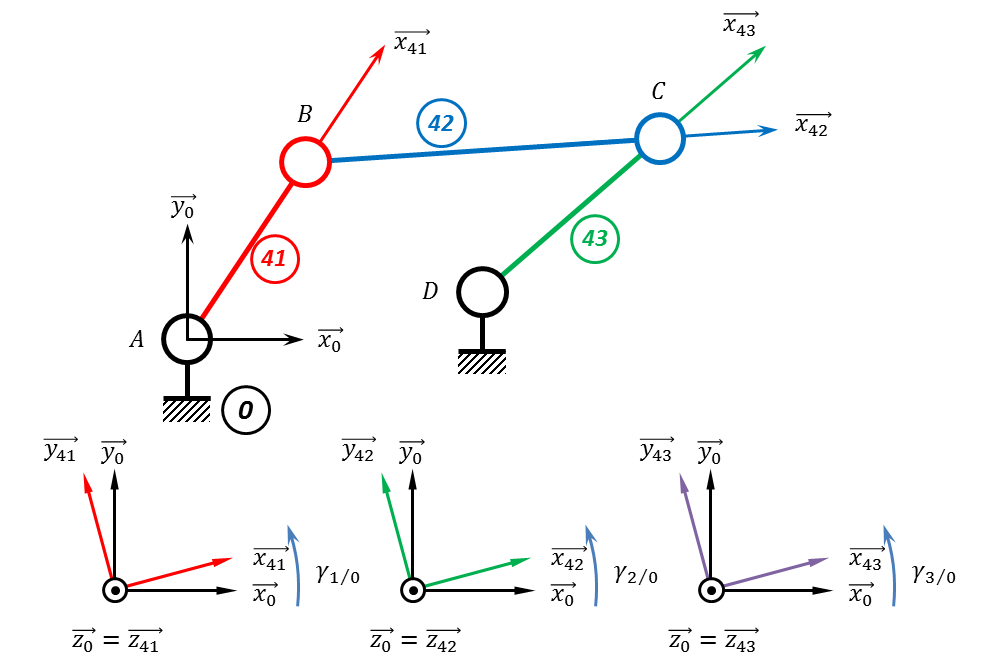
\includegraphics[width=\linewidth]{A6_3barres}
\end{center}

On donne : 

\begin{minipage}[c]{.45\linewidth}
\begin{itemize}
\item [$\bullet$] $\vect{AB}=L_1\vect{x_{41}}$;
\item [$\bullet$] $\vect{BC}=L_2\vect{x_{42}}$;
\end{itemize}
\end{minipage}\hfill
\begin{minipage}[c]{.45\linewidth}
\begin{itemize}
\item [$\bullet$] $\vect{DC}=L_3\vect{x_{43}}$;
\item [$\bullet$] $\vect{AD}=a\vect{x_{0}}+b\vect{y_{0}}$.
\end{itemize}
\end{minipage}

\fi
\subparagraph{}
\textit{Établir une relation géométrique entre $\gamma_1$ et $\gamma_3$. Cette relation pourra faire intervenir les différents paramètres constants ($a$, $b$, $L_1$, $L_2$, $L_3$). On ne devra pas voir apparaître $\gamma_2$.}

\ifprof
\begin{corrige}
En écrivant la fermeture de chaîne géométrique, on a : 

\begin{eqnarray*}
&& \vect{AB}+\vect{BC}+\vect{CD} + \vect{DA} = \vect{0} \\
& \Longleftrightarrow& L_1\vect{x_{41}} + L_2\vect{x_{42}} - L_3\vect{x_{43}}
- a\vect{x_{0}}-b\vect{y_{0}} = \vect{0}\\
& \Longleftrightarrow&  
L_1\left(\cos\gamma_{1}\vect{x_0}+ \sin\gamma_{1}\vect{y_0}\right) + L_2\left(\cos\gamma_{2}\vect{x_0}+ \sin\gamma_{2}\vect{y_0}\right)
-L_3\left(\cos\gamma_{3}\vect{x_0}+ \sin\gamma_{3}\vect{y_0}\right)
- a\vect{x_{0}}-b\vect{y_{0}} = \vect{0}\\
\end{eqnarray*}
En projetant respectivement cette expression sur $\vect{x_0}$ et $\vect{y_0}$, on a : 
$$
\left\{
\begin{array}{l}
L_1 \cos\gamma_{1} + L_2 \cos\gamma_{2} 
-L_3\cos\gamma_{3} - a= 0\\
L_1 \sin\gamma_{1} + L_2 \sin\gamma_{2}
-L_3 \sin\gamma_{3} -b=0
\end{array}
\right.
\Longleftrightarrow
\left\{
\begin{array}{l}
L_2 \cos\gamma_{2} =L_3\cos\gamma_{3}- L_1 \cos\gamma_{1} + a  \\
L_2 \sin\gamma_{2} = L_3 \sin\gamma_{3}-L_1 \sin\gamma_{1} + b
\end{array}
\right.
$$

On a donc : 
\begin{eqnarray*}
L_2^2 &=& \left( L_3\cos\gamma_{3}- L_1 \cos\gamma_{1} + a  \right)^2
+ \left( L_3 \sin\gamma_{3}-L_1 \sin\gamma_{1} + b\right)^2 \\
L_2^2 &=& 
L_3^2\cos^2\gamma_{3}+ L_1^2 \cos^2\gamma_{1} + a^2 \\
&&-2  L_3 L_1\cos\gamma_{3} \cos\gamma_{1}
+2 b L_3 \cos\gamma_{3}
-2bL_1 \cos\gamma_{1}\\
&&+L_3^2 \sin^2\gamma_{3}+ L_1^2 \sin^2\gamma_{1} + b^2 \\
&&-2  L_3 L_1 \sin\gamma_{3} \sin\gamma_{1}
+2 b L_3 \sin\gamma_{3}
-2bL_1 \sin\gamma_{1}\\
& = & L_3^2+ L_1^2  + a^2+ b^2  
-2  L_3 L_1\left( \cos\gamma_{3} \cos\gamma_{1} + \sin\gamma_{3} \sin\gamma_{1} \right)\\
&& +2 b L_3 \left( \cos\gamma_{3} + \sin\gamma_{3}\right)
-2bL_1 \left( \cos\gamma_{1} + \sin\gamma_{1}\right)\\
\end{eqnarray*}
\end{corrige}
\else \fi





\ifprof
%\end{multicols}
\else
\end{multicols}
\fi
